\documentclass[journal]{IEEEtran}
\usepackage{blindtext}
\usepackage{graphicx}
\usepackage{cite}
\usepackage{multirow}
\usepackage{booktabs}
\usepackage{siunitx}
\usepackage[pdftex,breaklinks,pdfauthor={MSD Team P17101},pdfcreator={Philip Linden},pdftitle={Prototype Arcjet Satellite Thruster}]{hyperref}

% cite.sty was written by Donald Arseneau
% V1.6 and later of IEEEtran pre-defines the format of the cite.sty package
% \cite{} output to follow that of IEEE. Loading the cite package will
% result in citation numbers being automatically sorted and properly
% "compressed/ranged". e.g., [1], [9], [2], [7], [5], [6] without using
% cite.sty will become [1], [2], [5]--[7], [9] using cite.sty. cite.sty's
% \cite will automatically add leading space, if needed. Use cite.sty's
% noadjust option (cite.sty V3.8 and later) if you want to turn this off.
% cite.sty is already installed on most LaTeX systems. Be sure and use
% version 4.0 (2003-05-27) and later if using hyperref.sty. cite.sty does
% not currently provide for hyperlinked citations.
% The latest version can be obtained at:
% http://www.ctan.org/tex-archive/macros/latex/contrib/cite/
% The documentation is contained in the cite.sty file itself.

% http://edge.rit.edu/edge/P17101/public/Home

\title{P17101: Prototype Arcjet Satellite Thruster}
\author{
  Philip~Linden$^{\dagger}$\thanks{$^{\dagger}$MEng Student, Department of Mechanical Engineering},
  James~Gandek$^{*}$\thanks{$^{*}$BS Student, Department of Mechanical Engineering},
  Dylan~Bruce$^{*}$,
  Matt~Giuffre$^{*}$,
  Anthony~Higgins$^{\ddagger}$\thanks{$^{\ddagger}$BS Student, Department of Electrical Engineering},
  David~Yin$^{\ddagger}$,
  Vince~Burolla$^{\dagger\dagger}$\thanks{$^{\dagger\dagger}$Project Adviser}
}
  % page header for pages other than cover page
  \markboth{P17101 Arcjet Thruster}%
  {Shell \MakeLowercase{\textit{et al.}}: Multidisciplinary Senior Design, RIT}

\begin{document}
\maketitle

% correct bad hyphenation here
\hyphenation{explor-ation explor-atory}

\begin{abstract}
A tabletop prototype of an arcjet electrothermal propulsion system was developed to supplement ongoing exploratory spacecraft development conducted by RIT Space Exploration (SPEX). The arcjet thruster demonstrates the degree of practicality in implementing electrothermal propulsion systems. The arcjet assembly generates an electrical arc across the thruster nozzle's throat, ionizing argon propellant in order to achieve a greater specific impulse compared to cold gas propulsion.
\end{abstract}

\section{Nomenclature}
\label{sec:nomenclature}
% List all symbols and subscripts used for any math equations.

\section{Introduction}
\label{sec:intro}
RIT Space Exploration (SPEX) provided a hypothetical use-case to serve as the foundation for this exploration into satellite propulsion.
SPEX's hypothetical mission objective is to design a communicaitons satellite that is capable of maintaining a polar geostationary orbit for 10 years.

In practice, satellites in Earth orbit for long-duration missions in excess of 5--25 years encounter perturbations to their trajectories over time from residual atmospheric and orbital particles, or from variations in Earth's gravity field.
These spacecraft perform short station-keeping maneuvers periodically to compensate for drift and orbital decay.

An electrothermal rocket engine is method of propulsion by which an inert gas stored at ambient temperature (cold gas) is released from a pressurized vessel or driven by a pump and heated electrically before being expelled out of a nozzle.
Two proven methods of electrothermal propulsion are \emph{resistojets}, which use conventional heat exchangers to heat the propellant, and \emph{arcjets}, which pass the propellant through an electrical arc to heat the gas.

Electrothermal propulsion is advantageous over conventional chemical or cold-gas rockets for use by long-life satellites since the engines may be small in size, have no moving parts, and are more efficient at the expense of thrust.
While resistojets and arcjets require more elecrical power than chemical rockets, for example, the electrical energy may be recovered over time by photovoltaic panels, for example, whereas propellant fuel is a finite resource for these spacecraft.

A tabletop prototype thruster was designed and tested to explore the feasibility of this type of system with less strict requirements compared to the limitations of building a flight-worthy system.
A tabletop version does not require integration with a spacecraft, and mass and spatial limitations are relaxed.

\section{Design Methodology}
\label{sec:method}
% Describe why an arcjet was selected over a resistojet.
In low power (\SI{1}{\kilo\watt}) applications, an arcjet offers up to 200\% gains in efficiency over a resistojet thruster~\cite{sutton}.
\autoref{fig:power-vs-isp} identifies the typical use cases and performance characteristics of arcjets compared to various other types of electrothermal thrusters.
Arcjets achieve a greater \emph{specific impulse} compared to resistojets but produce less thrust.
Thus a maneuver would take a longer amount of time using an arcjet but would consume less propellant overall for the same maneuver as compared to a resistojet.
\begin{figure}[hbp]
  \centering
  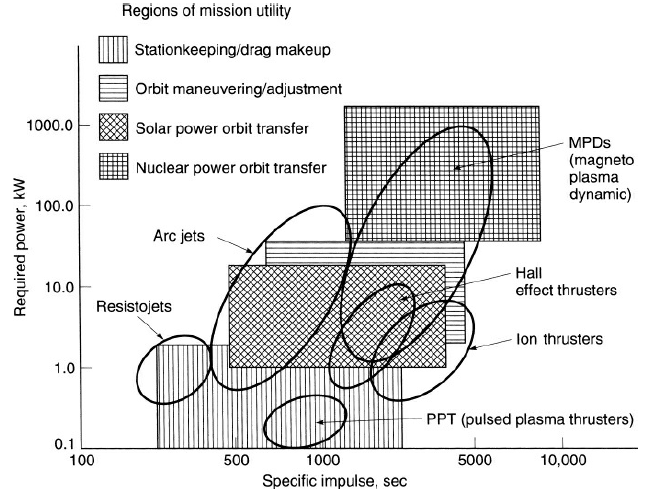
\includegraphics[width=\linewidth]{img/power-vs-isp_sutton}
  \caption[Types of electrothermal propulsion]{Types of electrothermal propulsion with respect to typical performance and mission utility.
  In the \SI{1}{\kilo\watt} range, arcjets typically have a higher specific impulse than resistojets. (Sutton~2010)
\label{fig:power-vs-isp}}
\end{figure}

\subsection{Gas Dynamics}
% Justify propellant selection (and explain paschen curve?)

% High level gas dynamics analysis
\begin{figure}[hbp]
  \centering
  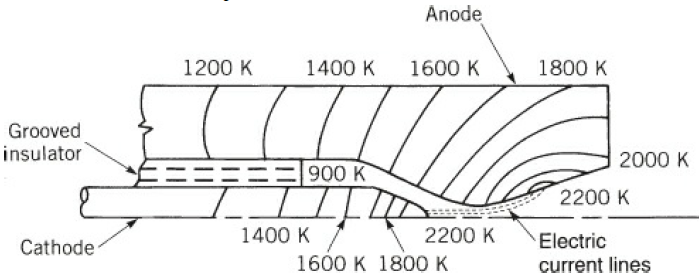
\includegraphics[width=\linewidth]{img/cross-section_sutton}
  \caption[Arcjet cross-section]{A cross sectional view of a typical arcjet shows the expected thermal profile in the anode (nozzle) and the expected location of the electric current. (Sutton~2010)
\label{fig:x-section-sutton}}
\end{figure}

\subsection{Power Conditioning}
% Explain how the PCU works

\subsection{Test Signal Amplification}
% Test stand theory

\section{System Overview}
% outline the main system architecture.

\subsection{Thruster Design}
% Describe the main components of the thruster and how they interact. Be sure to include material selection justifications. Show some basic analysis and predictions for performance with justification.

\subsection{Power Conditioning Unit}
% Describe the inputs and desired outputs of the unit. Explain the theoretical justification behind the HV/HC approach. Describe the approach in theoretical terms and list practical limitations.

\section{Testing}
% Describe the basic test plan in broad terms and how we approached testing. Describe the setup within the engine test cell and how the user interacts with the system.

\subsection{Test Stand}
% Explain the physical apparatus that measures the system's outputs. Describe the interactions between the thruster and the test stand. Justify instrumentation selection.

\subsection{Data Acquisition}
% Explain the DAQ hookup and justification for the DAQ, and limitations to that choice. Show and describe the VI\@.

\subsection{Safety Measures}
% Describe risk management in more detail. Consider ommitting this section~\cite{linden}.

\section{Results}
% Show results and how they compare to our predictions. Describe any failures and the problem solving process that occurred.

\section{Conclusions and Recommendations}
% Evaluate the success of the project and make recommendations for improving it.

\section*{Acknowledgments}
The team thanks Vince Burolla for his unwavering support, Dr.\ Dorin Patru and Dr.\ Chris Hoople for their technical advice; Formula SAE, the Multidisciplinary Senior Design Department, and the Kate Gleason College of Engineering for their resources and workspaces; RIT Space Exploration and Boeing for sponsoring this project.

\bibliographystyle{IEEEtran}
\bibliography{p17101}

\end{document}
